\begin{figure}[h!]
	\centering
	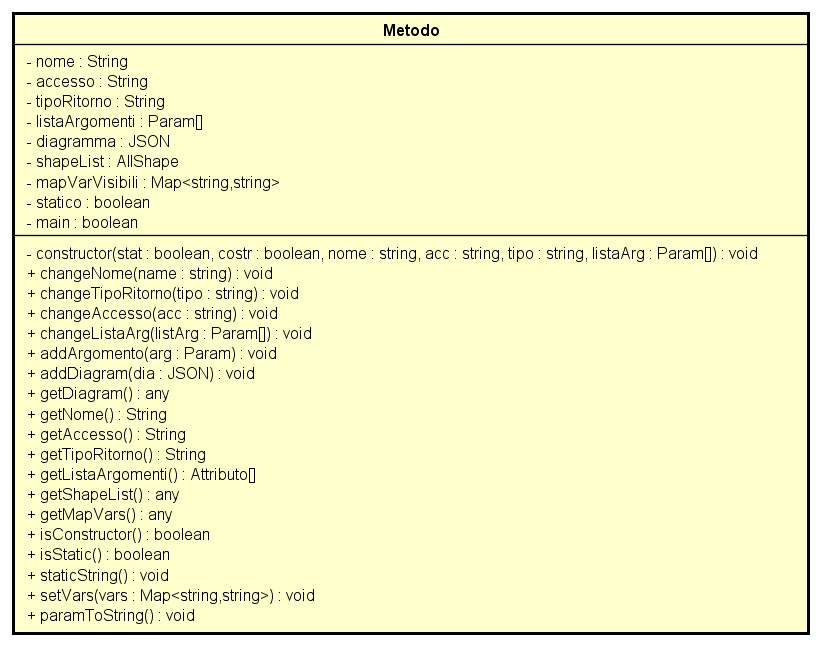
\includegraphics[scale=0.8]{res/sections/SpecificaFrontEnd/Services/Disegnetti/metodo.png}
	\caption{Diagramma della classe Metodo}
\end{figure}

\begin{itemize}
	\item \textbf{Descrizione:}\\
	
	\item \textbf{Utilizzo:}\\
	
	\item \textbf{Metodi:}
		\begin{itemize}
			\item \emph{-nome: string}\\
    		Nome del metodo
    		\item \emph{-accesso: string}\\
    		Visibilità del metodo
    		\item \emph{-tipoRitorno: string}\\
    		Tipo di ritorno del metodo
    		\item \emph{-listaArgomenti: Param[]}\\
    		Lista di argomenti del metodo
    		\item \emph{-diagramma: JSON}\\
    		
    		\item \emph{-shapeList: AllShape}\\
    		
    		\item \emph{-mapVarVisibili: Map<string, string>}\\
    		
    		\item \emph{-statico: boolean}\\
    		True se il metodo è marcato static
    		\item \emph{-main: boolean}\\
    		True se il metodo è main
		\end{itemize}
	\item \textbf{Metodi:}
		\begin{itemize}
			\item \emph{-constructor(stat: boolean, costr: boolean, nome: string, acc: string, tipo: string, listaArg: Param[])}\\
    		Costruisce il metodo\\
    		\textbf{Parametri:}
    		\begin{itemize}
    			\item \emph{stat: boolean}\\
    			True se il metodo deve essere marcato static
    			\item \emph{costr: boolean}\\
    			True se il metodo è un costruttore
    			\item \emph{nome: string}\\
    			Nome del metodo da creare
    			\item \emph{acc: string}\\
    			Visibilità del metodo
    			\item \emph{tipo: string}\\
    			Tipo di ritorno del metodo
    			\item \emph{listaArg: Param[]}\\
    			Lista degli argomenti del metodo
    		\end{itemize}
    		\item \emph{+changeNome(name: string)}\\
    		Modifica il nome del metodo selezionato\\
    		\textbf{Parametri:}
    		\begin{itemize}
    			\item \emph{name: string}\\
    			Nuovo nome del metodo
    		\end{itemize}
    		\item \emph{+changeTipoRitorno(tipo: string)}\\
    		Modifica il tipo di ritorno del metodo\\
    		\textbf{Parametri:}
    		\begin{itemize}
    			\item \emph{tipo: string}\\
    			Tipo di ritorno
    		\end{itemize}
    		\item \emph{+changeAccesso(acc: string)}\\
    		Modifica la visibilità del metodo\\
    		\textbf{Parametri:}
    		\begin{itemize}
    			\item \emph{acc: string}\\
    			Visibilità del metodo
    		\end{itemize}
    		\item \emph{+changeListaArg(listArg: Param[])}\\
    		Modifica la lista degli argomenti del metodo\\
    		\textbf{Parametri:}
    		\begin{itemize}
    			\item \emph{listArg: Param[]}\\
    			Lista degli argomenti
    		\end{itemize}
    		\item \emph{+addArgomento(arg: Param)}\\
    		Aggiunge un argomento al metodo\\
    		\textbf{Parametri:}
    		\begin{itemize}
    			\item \emph{arg: Param}\\
    			Argomento da aggiungere
    		\end{itemize}
    		\item \emph{+addDiagram(dia: JSON)}\\
    		Assegna il file JSON all'attributo diagramma della classe\\
    		\textbf{Parametri:}
    		\begin{itemize}
    			\item \emph{dia: JSON}\\
    			File JSON
    		\end{itemize}
    		\item \emph{+getDiagram()}\\
    		Ritorna l'attributo diagramma
    		\item \emph{+getNome()}\\
    		Ritorna il nome del metodo
    		\item \emph{+getAccesso()}\\
    		Ritorna la visibilità del metodo
    		\item \emph{+getTipoRitorno()}\\
    		Ritorna il tipo di ritorno del metodo
    		\item \emph{+getListaArgomenti()}\\
    		Ritorna la lista degli argomenti del metodo
    		\item \emph{+getShapeList()}\\
    		
    		\item \emph{+getMapVars()}\\
    		
    		\item \emph{+isConstructor()}\\
    		
    		\item \emph{+isStatic()}\\
    		
    		\item \emph{+staticString()}\\
    		
    		\item \emph{+setVars(vars: Map<string, string>)}\\
    		\\
    		\textbf{Parametri:}
    		\begin{itemize}
    			\item \emph{vars: Map<string, string>}\\
    			
    		\end{itemize}
    		\item \emph{+paramToString()}\\
    		
    	\end{itemize}
\end{itemize}